\documentclass[9pt]{beamer}
\mode<presentation>

% ============================================================
% GENESIS IDEATHON: FINAL PRESENTATION TEMPLATE
% Edit the team details and the content inside each slide.
% Keep the setup section unchanged unless you want to customise
% the visual style of the presentation.
% ============================================================

% -------------------- THEME AND COLOURS ---------------------
\usetheme{Madrid}
\usecolortheme{default}
\usefonttheme{structurebold}
\setbeamercovered{invisible}
\setbeamertemplate{navigation symbols}{}

% Genesis green palette
\definecolor{GenesisGreen}{RGB}{35,105,70}
\definecolor{GenesisDarkGreen}{RGB}{22,75,51}
\definecolor{GenesisLightGreen}{RGB}{225,241,231}
\definecolor{GenesisCream}{RGB}{250,248,240}

% Apply the Genesis palette to Beamer elements
\setbeamercolor{structure}{fg=GenesisGreen}
\setbeamercolor{palette primary}{bg=GenesisDarkGreen,fg=white}
\setbeamercolor{palette secondary}{bg=GenesisGreen,fg=white}
\setbeamercolor{palette tertiary}{bg=GenesisDarkGreen,fg=white}
\setbeamercolor{palette quaternary}{bg=GenesisGreen,fg=white}
\setbeamercolor{frametitle}{bg=GenesisLightGreen,fg=GenesisDarkGreen}
\setbeamercolor{title}{fg=GenesisDarkGreen}
\setbeamercolor{block title}{bg=GenesisGreen,fg=white}
\setbeamercolor{block body}{bg=GenesisLightGreen,fg=black}
\setbeamercolor{item}{fg=GenesisGreen}
\setbeamercolor{section in toc}{fg=GenesisDarkGreen}
\setbeamercolor{subsection in toc}{fg=GenesisGreen}
\setbeamercolor{normal text}{fg=black,bg=white}
\setbeamercolor{author in head/foot}{bg=GenesisLightGreen,fg=GenesisDarkGreen}
\setbeamercolor{date in head/foot}{bg=GenesisLightGreen,fg=GenesisDarkGreen}

% ------------------------- PACKAGES -------------------------
\usepackage{graphicx}
\usepackage{amsfonts}
\usepackage{amsmath}
\usepackage{amssymb}
\usepackage{amsthm}
\usepackage{mathtools}
\usepackage{hyperref}
\usepackage[utf8]{inputenc}
\usepackage[T1]{fontenc}
\usepackage{lmodern}
\usepackage{tikz}
\usetikzlibrary{calc}
\usepackage[absolute,overlay]{textpos}
\usepackage{array}
\usepackage{colortbl}

% ---------------------- LAYOUT TUNING -----------------------
% Shared left/right margin: slide text, frame titles, and the
% footer all line up on the same vertical edge.
\newlength{\GenesisMargin}
\setlength{\GenesisMargin}{0.9cm}
\setbeamersize{text margin left=\GenesisMargin,text margin right=\GenesisMargin}

% Comfortable line and paragraph spacing
\linespread{1.12}
\setlength{\parskip}{0pt}

% Bullets: clean markers and more space between items
\setbeamertemplate{itemize item}[square]
\setbeamertemplate{itemize subitem}[circle]
\setbeamerfont{itemize/enumerate body}{size=\normalsize}
\setlength{\leftmargini}{1.4em}
\makeatletter
\def\@listi{\leftmargin\leftmargini
  \topsep 6pt plus 2pt minus 2pt
  \parsep 0pt
  \itemsep 10pt plus 3pt minus 3pt}
\let\@listI\@listi
\makeatother

% Rounded blocks (used for highlighted content)
\setbeamertemplate{blocks}[rounded][shadow=false]
\setbeamerfont{block title}{size=\normalsize,series=\bfseries}

% Frame title: fixed-height band with an accent rule, so the
% corner logo sits centred inside it on every content slide.
\setbeamerfont{frametitle}{size=\Large,series=\bfseries}
\setbeamertemplate{frametitle}{%
  \nointerlineskip
  \begin{beamercolorbox}[wd=\paperwidth,ht=0.58cm,dp=0.3cm,leftskip=\GenesisMargin]{frametitle}%
    \usebeamerfont{frametitle}\insertframetitle
  \end{beamercolorbox}%
  \nointerlineskip
  \begin{beamercolorbox}[wd=\paperwidth,ht=1.4pt,dp=0pt]{palette secondary}\end{beamercolorbox}%
}

% Numbered entries in the outline
\setbeamertemplate{section in toc}[sections numbered]
\setbeamerfont{section in toc}{size=\normalsize,series=\mdseries}

% --------------------- TEAM INFORMATION ---------------------
% Update these two commands. They appear in the footer of content slides.
\newcommand{\TeamNumber}{GEN26-A0H-I096}
\newcommand{\TeamName}{Dark Mod Devs}

% ------------------------- FOOTER ---------------------------
% Team number and team name appear at the bottom-left.
% The presentation date appears at the bottom-right.
\setbeamertemplate{footline}{%
  \leavevmode%
  \hbox{%
    \begin{beamercolorbox}[wd=.72\paperwidth,ht=3.0ex,dp=1.3ex,leftskip=\GenesisMargin]{author in head/foot}%
      \usebeamerfont{author in head/foot}\TeamNumber\ \textbar\ \TeamName
    \end{beamercolorbox}%
    \begin{beamercolorbox}[wd=.28\paperwidth,ht=3.0ex,dp=1.3ex,rightskip=\GenesisMargin]{date in head/foot}%
      \usebeamerfont{date in head/foot}\hfill\insertdate
    \end{beamercolorbox}%
  }%
}

% ---------------- PRESENTATION DETAILS ---------------------
% Replace these values with your team's actual information.
\title[Genesis Ideathon]{Genesis Ideathon: Final Presentation}
\author{Team ID: \textit{GEN26-A0H-I096}\\[0.2cm]
Team Name: \textit{Dark Mod Devs}\\[0.2cm]
Domain: \textit{Digital Technologies, AI \& Cyber Security}}
\institute{Amrita Vishwa Vidyapeetham, Coimbatore Campus}
\date{11th October 2026}

% -------------------------- LOGOS --------------------------
% The title slide displays all three logos.
% These filenames match the files shown in your Overleaf project.
% Each logo is vertically centred on the same line.
% Usage: \GenesisTitleLogo[height]{file}  (default height 1.35cm)
\newcommand{\GenesisTitleLogo}[2][1.35cm]{%
  \raisebox{-0.5\height}{\includegraphics[height=#1]{#2}}}
\titlegraphic{%
  \GenesisTitleLogo{reference_logos/Amrita_Vishwa_Vidyapeetham_Logo.png}%
  \hspace{0.7cm}%
  \GenesisTitleLogo[1.0cm]{reference_logos/iic_logo.png}%
  \hspace{0.7cm}%
  \GenesisTitleLogo[1.0cm]{reference_logos/genesis-iic.png}%
}

% Genesis logo at the top-right of content slides only.
% The title slide and outline slide do not use this logo placement.
% It is right-aligned to the slide margin and centred in the title band.
\newcommand{\GenesisCornerLogo}{%
  \begin{textblock*}{3cm}(\dimexpr\paperwidth-3cm-\GenesisMargin\relax,0.12cm)
    \raggedleft\includegraphics[height=0.64cm]{reference_logos/genesis-iic.png}
  \end{textblock*}%
}

% Title page: logos on top, then the title and team details (no footer).
\setbeamertemplate{title page}{%
  % Accent band along the top edge
  \begin{textblock*}{\paperwidth}(0cm,0cm)
    \begin{beamercolorbox}[wd=\paperwidth,ht=0.16cm,dp=0pt]{palette primary}\end{beamercolorbox}
  \end{textblock*}%
  \begin{minipage}[t][0.9\textheight][t]{\textwidth}
    % ---- Logos ----
    \vspace*{0.45cm}
    \begin{center}
      \inserttitlegraphic
    \end{center}
    \vspace{0.1cm}
    {\color{GenesisLightGreen}\rule{\textwidth}{1.2pt}\par}
    % ---- Title ----
    \vspace{0.3cm}
    \raggedright
    {\color{GenesisGreen}\rule{0.22\textwidth}{2.5pt}\par}
    \vspace{0.25cm}
    {\usebeamerfont{title}\usebeamercolor[fg]{title}\LARGE\bfseries\inserttitle\par}
    % ---- Team details ----
    \vspace{0.4cm}
    
\begin{tikzpicture}
      \node[fill=GenesisLightGreen,rounded corners=4pt,inner sep=0.35cm,
            text width=\dimexpr\textwidth-0.7cm\relax,align=left,
            font=\large] (card) {\insertauthor};
      \fill[GenesisGreen,rounded corners=1.5pt]
        ([xshift=0pt]card.north west) rectangle ([xshift=3pt]card.south west);
    \end{tikzpicture}\par
    \vspace{0.45cm}
    {\normalsize{\color{GenesisDarkGreen}\insertinstitute}\hfill\textbf{Date:} \insertdate\par}
  \end{minipage}%
}

% ------------------------- TABLES ---------------------------
% Column types: C = centred, L = left-aligned (both vertically centred).
\newcolumntype{C}[1]{>{\centering\arraybackslash}m{#1}}
\newcolumntype{L}[1]{>{\raggedright\arraybackslash}m{#1}}
% Header row and alternating body rows in the Genesis palette.
\newcommand{\GenesisHeadRow}{\rowcolor{GenesisGreen}}
\newcommand{\GenesisHead}[1]{\textcolor{white}{\textbf{#1}}}
\newcommand{\GenesisRowA}{\rowcolor{GenesisLightGreen}}
\newcommand{\GenesisRowB}{\rowcolor{GenesisLightGreen!40}}
% Wrapper: white rules between cells and roomy rows.
\newenvironment{GenesisTable}[1]{%
  \begin{center}
  \renewcommand{\arraystretch}{1.9}%
  \setlength{\tabcolsep}{4pt}%
  \arrayrulecolor{white}\setlength{\arrayrulewidth}{1.2pt}%
  \begin{tabular}{#1}}{%
  \end{tabular}
  \end{center}}

% Highlight card for the Yukthi ID on the last slide.
\newcommand{\GenesisIDCard}[2]{%
  \begin{tikzpicture}
    \node[fill=white,draw=GenesisGreen,line width=1.2pt,rounded corners=6pt,
          minimum width=7.6cm,minimum height=2.3cm,align=center,
          text=GenesisDarkGreen,font=\Huge\bfseries] (id) {#2};
    \node[fill=GenesisGreen,text=white,rounded corners=4pt,
          inner xsep=0.45cm,inner ysep=0.14cm,font=\normalsize\bfseries]
          at (id.north) {#1};
  \end{tikzpicture}%
}

% Placeholder box for the architecture / use-case diagram.
\newcommand{\GenesisDiagramBox}[1]{%
  \begin{tikzpicture}
    \node[draw=GenesisGreen,dashed,line width=0.8pt,rounded corners=4pt,
          fill=GenesisLightGreen!45,text=GenesisDarkGreen,
          text width=0.86\textwidth,minimum height=2.9cm,align=center,
          inner sep=6pt]{#1};
  \end{tikzpicture}%
}

% ============================================================
% DOCUMENT START
% ============================================================
\begin{document}

% ------------------------- TITLE SLIDE ----------------------
% Three logos on top, then team ID, team name, and domain.
\begin{frame}[plain]
  \titlepage
\end{frame}

% ------------------------- OUTLINE --------------------------
% This extra slide is separate from the 12 required content slides.
% It intentionally has no Genesis corner logo and no footer.
% (The footer is switched off in the group around the frame.)
{
\setbeamertemplate{footline}{}
\begin{frame}{Presentation Outline}
  \begin{columns}[T,onlytextwidth]
    \begin{column}{0.48\textwidth}
      \tableofcontents[sections={1-6}]
    \end{column}
    \begin{column}{0.48\textwidth}
      \tableofcontents[sections={7-12}]
    \end{column}
  \end{columns}
\end{frame}
}

% ============================================================
% SLIDE 1: PROBLEM STATEMENT
% ============================================================
\section{Problem Statement}
\begin{frame}{Problem Statement}
  \GenesisCornerLogo
  \begin{beamercolorbox}[rounded=true,sep=0.35cm,wd=\dimexpr\textwidth-0.7cm\relax]{block body}
    \textbf{Detecting and Disrupting Mule-Account Networks Behind Digital Payment Fraud}\par\vspace{0.25cm}
    When someone is scammed on UPI, the money is split across a few ordinary people's accounts and withdrawn within minutes. Every bank sees only its own account, so nobody sees the whole chain in time to stop it.
  \end{beamercolorbox}
\end{frame}

% ============================================================
% SLIDE 2: PROBLEM UNDERSTANDING
% ============================================================
\section{Problem Understanding}
\begin{frame}{Problem Understanding}
  \GenesisCornerLogo
  \begin{itemize}
    \item \textbf{Who:} everyday UPI users, especially first-time digital users such as parents, grandparents, small shop owners and daily wage workers. Students tempted to lend their account for commission are part of the problem too.
    \item \textbf{Cause:} UPI is instant and cannot be reversed, and each bank sees only its own account.
    \item \textbf{Effect:} complaints rose from 13.1 lakh (2023) to 24.02 lakh (2025), with Rs.\,22,495 crore reported lost in 2025. \textit{\small Source: MHA replies in Parliament, 2026.}
  \end{itemize}
\end{frame}

% ============================================================
% SLIDE 3: EXISTING GAPS & CHALLENGES
% ============================================================
\section{Existing Gaps \& Challenges}
\begin{frame}{Existing Gaps \& Challenges}
  \GenesisCornerLogo
  \begin{itemize}
    \item \textbf{Bank rule-based checks:} fixed rules, many false alerts, and each bank sees only its own accounts.
    \item \textbf{1930 helpline, CFCFRMS and I4C Suspect Registry:} action starts only after the victim reports, and the registry covers only identifiers already known to be bad.
    \item \textbf{RBI MuleHunter.AI:} strong at flagging single accounts, but as far as public information shows, it does not follow a live chain across banks.
    \item \textbf{Unsolved:} a real-time cross-bank view of the chain with a soft, reversible response.
  \end{itemize}
\end{frame}

% ============================================================
% SLIDE 4: OUR PROPOSED SOLUTION
% ============================================================
\section{Our Proposed Solution}
\begin{frame}{Our Proposed Solution}
  \GenesisCornerLogo
  \begin{itemize}
    \item \textbf{Core idea:} \emph{ChainBreak}, a shared signal layer where banks share only masked account IDs and risk scores. No customer data leaves a bank.
    \item \textbf{How it works:} a graph model finds mule chains (fast pass-through, many-to-one, one-to-many, brand new accounts). Federated learning lets banks improve it together without sharing raw data.
    \item \textbf{Response:} alert, small delay or extra confirmation, short hold on that chain only, then human review with an auto-release timer.
    \item \textbf{Value:} more of the victim's money is stopped midway, and honest users are delayed, not blocked.
  \end{itemize}
\end{frame}

% ============================================================
% SLIDE 5: TECHNICAL APPROACH
% ============================================================
\section{Technical Approach}
\begin{frame}{Technical Approach}
  \GenesisCornerLogo
  \begin{center}
  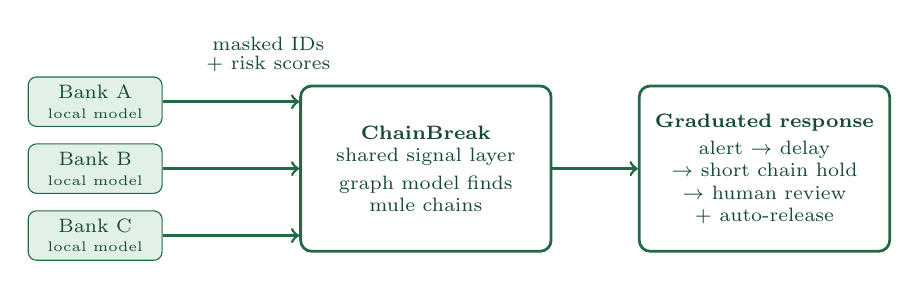
\begin{tikzpicture}[font=\scriptsize,
      box/.style={draw=GenesisGreen,fill=GenesisLightGreen,rounded corners=3pt,
                  align=center,inner sep=3pt,text=GenesisDarkGreen},
      big/.style={draw=GenesisGreen,fill=white,line width=1pt,rounded corners=4pt,
                  align=center,inner sep=4pt,text=GenesisDarkGreen},
      arr/.style={->,line width=1pt,color=GenesisGreen}]
    \node[box,minimum width=1.7cm,minimum height=0.6cm] (a) at (0,0.85) {Bank A\\[-1pt]\tiny local model};
    \node[box,minimum width=1.7cm,minimum height=0.6cm] (b) at (0,0)    {Bank B\\[-1pt]\tiny local model};
    \node[box,minimum width=1.7cm,minimum height=0.6cm] (c) at (0,-0.85){Bank C\\[-1pt]\tiny local model};
    \node[big,text width=2.9cm,minimum height=2.1cm] (s) at (4.2,0)
      {\textbf{ChainBreak}\\shared signal layer\\[2pt]graph model finds\\mule chains};
    \node[big,text width=2.9cm,minimum height=2.1cm] (r) at (8.5,0)
      {\textbf{Graduated response}\\[2pt]alert $\rightarrow$ delay\\$\rightarrow$ short chain hold\\$\rightarrow$ human review\\+ auto-release};
    \draw[arr] (a.east) -- ($(s.west)+(0,0.85)$);
    \draw[arr] (b.east) -- (s.west);
    \draw[arr] (c.east) -- ($(s.west)+(0,-0.85)$);
    \draw[arr] (s.east) -- (r.west);
    \node[align=center,text=GenesisDarkGreen] at (2.2,1.45) {masked IDs\\[-1pt]+ risk scores};
  \end{tikzpicture}
  \end{center}
  \vspace{-0.1cm}
  \begin{center}
    \small Banks train locally and send only masked signals; the shared layer links accounts across banks and triggers a gentle, reversible response.
  \end{center}
  \vspace{0.05cm}
  \begin{beamercolorbox}[rounded=true,sep=0.25cm,wd=\dimexpr\textwidth-0.5cm\relax]{block body}
    \small\textbf{Tech Stack}\par\vspace{0.1cm}
    \begin{tabular}{@{}>{\raggedright\arraybackslash}p{0.36\textwidth}>{\raggedright\arraybackslash}p{0.50\textwidth}@{}}
      \textbf{Frontend:} React dashboard & \textbf{Database:} Graph database, NetworkX \\[0.08cm]
      \textbf{Backend:} Python, FastAPI & \textbf{AI/ML:} PyTorch Geometric, Flower (federated), hashing/masking
    \end{tabular}
  \end{beamercolorbox}
\end{frame}

% ============================================================
% SLIDE 6: INNOVATION & UNIQUENESS
% ============================================================
\section{Innovation \& Uniqueness}
\begin{frame}{Innovation \& Uniqueness}
  \GenesisCornerLogo
  \begin{itemize}
    \item \textbf{What is new:} it follows a money chain across banks in real time using only masked IDs and risk scores.
    \item \textbf{Why it suits the problem:} federated learning respects privacy and competition rules while every bank still contributes to one shared model.
    \item \textbf{Key differentiator:} detection by chain behaviour, so brand new mule accounts can be caught, plus a reversible response where every hold releases itself unless a reviewer confirms it.
  \end{itemize}
\end{frame}

% ============================================================
% SLIDE 7: FEASIBILITY & SCALABILITY
% ============================================================
\section{Feasibility \& Scalability}
\begin{frame}{Feasibility \& Scalability}
  \GenesisCornerLogo
  \begin{itemize}
    \item \textbf{Feasibility:} the prototype needs only laptops, free open-source tools (Python, PyTorch Geometric, NetworkX, Flower, FastAPI, React) and synthetic transaction data, with a mentor or bank fraud officer to check our assumptions.
    \item \textbf{Scalability:} one local server at each bank plus one secure shared hub; later NPCI, a few banks and I4C as partners.
    \item \textbf{Risks:} real bank data cannot be shared, so results are on simulated data and need validation with partners. Wrong holds are limited by short, chain-only holds with auto-release and human review.
  \end{itemize}
\end{frame}

% ============================================================
% SLIDE 8: COST FOR PRODUCT
% ============================================================
\section{Cost for Product}
\begin{frame}{Cost for Product (Optional)}
  \GenesisCornerLogo
  \begin{itemize}
    \item Development cost: no software licence cost for the prototype (open-source tools, team laptops).
    \item Hosting cost: a cloud server (GPU optional) to train the graph model; amount depends on usage and will be scoped with partners.
    \item Estimated total: minimal for the prototype. Production cost to be estimated with NPCI and partner banks.
  \end{itemize}
\end{frame}

% ============================================================
% SLIDE 9: USE CASES
% ============================================================
\section{Use Cases}
\begin{frame}{Use Cases}
  \GenesisCornerLogo
  \begin{itemize}
    \item \textbf{Use case 1, a first-time UPI user:} a scam payment is split across three mule accounts in different banks. ChainBreak links them, delays onward transfers and holds the chain, so most of the money is stopped before cash-out.
    \item \textbf{Use case 2, a student lending an account:} money passes through the account within seconds. The pass-through pattern raises the risk score, triggering extra confirmation, a short hold and a reviewer check.
    \item \textbf{Use case 3, a genuine shopkeeper on a festival day:} many small incoming payments look like a many-to-one pattern. The low score triggers only a small delay, and it releases automatically, so there is no freeze.
  \end{itemize}
\end{frame}

% ============================================================
% SLIDE 10: IMPACTS AND BENEFITS
% ============================================================
\section{Impacts and Benefits}
\begin{frame}{Impacts and Benefits}
  \GenesisCornerLogo
  \begin{itemize}
    \item \textbf{Users:} victims keep more of their money, honest users and shops are not blocked, and people trust UPI more.
    \item \textbf{Social and economic:} banks lose less and get fewer complaints, and police see the whole chain instead of pieces.
    \item \textbf{Measurable targets (on simulated data):} catch most mule chains before the last withdrawal, place a hold within about a minute of detection, and keep wrong holds on genuine accounts very low.
  \end{itemize}
\end{frame}

% ============================================================
% SLIDE 11: SUSTAINABLE DEVELOPMENT GOALS
% ============================================================
\section{Sustainable Development Goals}
\begin{frame}{Sustainable Development Goals (SDGs)}
  \GenesisCornerLogo
  \begin{GenesisTable}{C{2.1cm}|C{2.25cm}|L{2.45cm}|L{2.95cm}}
    \GenesisHeadRow
    \GenesisHead{SDG Number} & \GenesisHead{Target Number} & \GenesisHead{Goal Name} & \GenesisHead{Connection} \\ \hline
    \GenesisRowA
    \textbf{SDG~16} & Target 16.4 & Peace, Justice and Strong Institutions & Disrupts illicit financial flows and gives police the whole chain \\ \hline
    \GenesisRowB
    \textbf{SDG~8} & Target 8.10 & Decent Work and Economic Growth & Builds trust in digital banking and protects honest users \\ \hline
    \GenesisRowA
    \textbf{SDG~9} & Target 9.1 & Industry, Innovation and Infrastructure & Makes payment infrastructure more resilient to fraud \\
  \end{GenesisTable}
\end{frame}

% ============================================================
% SLIDE 12: INDIVIDUAL MEMBER CONTRIBUTION
% ============================================================
\section{Individual Member Contribution}
\begin{frame}{Individual Member Contribution}
  \GenesisCornerLogo
  \begin{GenesisTable}{C{3.5cm}|L{6.3cm}}
    \GenesisHeadRow
    \GenesisHead{Member} & \GenesisHead{Contribution or responsibility} \\ \hline
    \GenesisRowA
    \textbf{Thiruvenkadesuwaran S} & Team leader: designs the slides and builds the prototype \\ \hline
    \GenesisRowB
    \textbf{K Prajit Raj} & Research lead: collects fraud data and facts, studies RBI/NPCI rules and existing solutions \\ \hline
    \GenesisRowA
    \textbf{Nithin V} & Solution and architecture lead: designs the cross-bank detection and holds, and makes the diagrams \\ \hline
    \GenesisRowB
    \textbf{Senthil Yohan N} & Presenter: writes the pitch story, practises it and delivers it \\
  \end{GenesisTable}
\end{frame}

% ============================================================
% LAST SLIDE: YUKTI ID
% This closing slide is not listed in the outline.
% ============================================================
\begin{frame}{Yukti ID}
  \GenesisCornerLogo
  % Replace "[Enter Yukthi ID]" with your team's Yukthi ID.
  \begin{center}
    \GenesisIDCard{Yukti ID}{IR2026-1051140 }
  \end{center}
\end{frame}

\end{document}